\newcommand{\cnt}{c}
\newcommand{\meas}{\epsilon}
\newcommand{\dt}{\Delta t}
\newcommand{\dtm}{\dt_{\meas}}
\newcommand{\dtc}{\dt_{\cnt}}
\newcommand{\Ncm}{{n_{\sfrac{\cnt}{\meas}}}}
\newcommand{\Nmnd}{{n_{\sfrac{\meas}{zc}}}}
\newcommand{\Nnd}{{n_{zc}}}
\newcommand{\Nm}{{n_{\meas}}}
\newcommand{\Ncnt}{{n_{\cnt}}}
\newcommand{\LTb}{\tau_b}
\newcommand{\LTd}{\tau_d}
\newcommand{\lamb}{\lambda_b}
\newcommand{\lamd}{\lambda_d}

\DeclareDocumentCommand{\mupp}{s}{\mu'_\phi\IfBooleanTF{#1}{}{(t_i)}}
\DeclareDocumentCommand{\mudpp}{s}{\mu''_{\phi^2}\IfBooleanTF{#1}{}{(t_i)}}
\newcommand{\pars}{\boldsymbol{\theta}}
\DeclareDocumentCommand{\XpctO}{m}{\Xpct{#1}[\pars_0]}
\DeclareDocumentCommand{\var}{O{}mo}{\mathrm{var}_{#1}\bkt*{#2\IfValueT{#3}{\vert~ #3}}}
\DeclareDocumentCommand{\Fisher}{O{}D(){\pars_0}}{I_{#1}(#2)}
\newcommand{\y}{\mathbf{y}}

\usepgfplotslibrary{fillbetween}

\chapter{Statistical modeling}\label{Apx:Stats}
In this appendix we analyze the standard error of the spin precession frequency in the storage ring
experiment for searching for the deuteron EDM. The main body of the analysis begins
in section~\ref{Apx:Stats:Detector_counting_rate}; section~\ref{Apx:Stats:Prelim} introduces some terms
(like sample Fisher information, Fisher information of a point), but it can be omitted.

Spin precession frequency is determined via fitting a harmonic signal 
$f(t) = a\cdot\sin(\w\cdot t + \delta)$ with constant parameters $(a,\w,\delta)$ to polarimetry data.
Polarimetry data are obtained by scattering the polarized beam on a carbon target. Two important aspects
of polarimetry are:
\begin{enumerate*}
	\item decrease of the number of beam particles at each measurement, and
	\item depolarization.
\end{enumerate*}

The first aspect motivates the search for a more optimal beam sampling strategy. In sampling the
beam polarization, most informative (in terms of frequency) are measurements made during a rapid change
in the signal(see section~\ref{Apx:Stats:Prelim} below). This was the basis of the idea to measure
polarization only when its vertical component crosses zero (frequency-modulated sampling): this way
sampling is done in the mose efficient manner, and the beam lifetime is extended. 

We must note, however, that the detector analyzing power is maximal in at the peaks of the measured signal,
and goes to zero in the nodes. This limits the opportunities of improvement of the sampling effectiveness
by modulated sampling: the most useful (for us) measurement are least certain, while the least useful can be
measured with most certainty.

It also affects the heteroskedasticity of the data: in our simulation we used a non-periodic measurement error
growth model~\cite[p.~18]{Eversmann:Thesis}, while the oscillations of the analyzing power introduce periodicity
into the error.

Depolarization is another factor restraining the usefulness of extending the beam lifetime; it
puts a much harder bound on the duration of the measurement cycle, and hence the standard error of the
frequency estimate obtained from a single cycle.


In the next sections we will introduce a detector counting rate model, the notion of cross section asymmetry,
and determine an adequate (in view of depolarization) length of the polarization measurement cycle.
We will also simulate experimental data in order to assess the potential of the frequency-modulated polarization samplign frequency.

\section{Preliminary analysis}\label{Apx:Stats:Prelim}

The probability of observing  the value $y_i \equiv y(t_i)$ when the expectation value is $\mu(t_i)$ and the error is Gaussian is
\begin{align*}
	f(y_i|\pars) &= \frac{1}{\sqrt{2\pi\nu}}\exp\bkt{-\frac12\frac{(y_i - \mu(t_i))^2}{\nu}}, \\
	\pars 		  &= (\nu,\omega,\phi),\\
	\mu(t_i) 	  &= N_0\bkt{1 + P\sin(\omega t_i + \phi)}.
\end{align*}

The likelihood of observing a set of observations $\y = (y_1,\dots, y_K)$, under the i.i.d. assumption, is the product of propabilities taken as a function of the parameters:
\begin{align*}
	\mathcal{L}(\pars|\y) &= \prod_i f(y_i|\pars),
\shortintertext{and the log-likelihood}
	\ell(\pars|\y) &= -\frac{K}{2}\log2\pi - \frac{K}{2}\log\nu - \frac{1}{2\nu}\sum_i\epsilon_i^2,
	~ \epsilon_i = y_i- \mu(t_i).
\end{align*}
The usual assumptions for the error term are zero expectation and strict exogeneity
\begin{align*}
	\XpctO{\epsilon_i} &= \XpctO{t_i\epsilon_i} = 0,
\intertext{and the relations between the mean's derivatives are}
	\mu'_\phi	&= N_0P\cos(\omega t + \phi), \\
	\mu'_\omega &= t\cdot\mu'_\phi, \epsilon'_\xi = -\mu'_\xi.
\end{align*}

%% The log-likelihood derivatives:
%% \begin{align*}
%% \ell'_\nu 		&= -\frac{K}{2\nu} + \frac{1}{2\nu^2}\sum_i\epsilon_i^2;  & \\
%% \ell'_\omega 	&= \frac1\nu\sum_i\mupp t_i\epsilon_i;  & \\
%% \ell'_\phi		&= \frac1\nu \sum_i \mupp\epsilon_i; & \\
%% %
%% \ell''_{\nu^2}		&= \frac{K}{2\nu^2} - \frac{1}{\nu^3}\sum_i\epsilon_i^2, 
%% 	&-\XpctO{\ell''_{\nu^2}} = \frac{K}{2\nu^2} - \frac{1}{\nu^3}\sum_i\nu = \frac{K}{2\nu^2};\\
%% \ell''_{\nu\omega}	&= -\frac{1}{\nu^2}\sum_i\mupp t_i\epsilon_i, 
%% 	&-\XpctO{\ell''_{\nu\omega}} = \frac{1}{\nu^2}\sum_i\mupp\XpctO{t_i\epsilon_i} = 0;\\
%% \ell''_{\nu\phi}	&= -\frac{1}{\nu^2}\sum_i\mupp \epsilon_i, 
%% 	&-\XpctO{\ell''_{\nu\phi}} = \frac{1}{\nu^2}\sum_i\mupp\XpctO{\epsilon_i} = 0; \\
%% \ell''_{\phi^2}		&= \frac1\nu\sum_i\bkt{\mudpp \epsilon_i - \bkt{\mupp}^2}, 
%% 	&-\XpctO{\ell''_{\phi^2}} = \frac1\nu\sum_i\bkt{\bkt{\mupp}^2 - \mudpp\XpctO{\epsilon_i}} = \frac1\nu\sum_i\bkt{\mupp}^2;\\
%% \ell''_{\phi\omega}	&= \frac1\nu\sum_i\bkt{\mudpp t_i\epsilon_i - \bkt{\mupp}^2t_i}, 
%% 	&-\XpctO{\ell''_{\phi\omega}} = \frac1\nu\sum_i\bkt{t_i\bkt{\mupp}^2 - \mudpp\XpctO{t_i\epsilon_i}} = \frac1\nu\sum_i t_i\bkt{\mupp}^2;\\
%% \ell''_{\omega^2}	&= \frac1\nu\sum_i\bkt{\mudpp t_i^2\epsilon_i - \bkt{\mupp t_i}^2},
%% 	& -\XpctO{\ell''_{\omega^2}} = \frac1\nu\sum_i\bkt{\bkt{t_i\mupp}^2 - \mudpp\XpctO{t_i^2\epsilon_i}} = \frac1\nu\sum_i\bkt{t_i\mupp}^2.
%% \end{align*}

\subsection{Variance of the frequency estimate}
After computing the lok-likelihood derivatives (and their expectation values), we can construct
the Fisher matrix
\[
\Fisher = \begin{pmatrix}
  \sfrac{K}{2\nu} & 0 								& 0 \\
  0 				& \sfrac1\nu\sum\bkt{t_i\mupp}^2	& \sfrac1\nu\sum t_i\bkt{\mupp}^2 \\
  0				& \sfrac1\nu\sum t_i\bkt{\mupp}^2	&\sfrac1\nu\sum\bkt{\mupp}^2
\end{pmatrix}.
\]
Its determinant
\newcommand{\STM}{\Omega}
\[
|\Fisher| = \frac{K}{2\nu^3}\underbrace{\bkt{\sum\bkt{t_i\mupp}^2\sum\bkt{\mupp}^2 - \bkt{\sum t_i\bkt{\mupp}^2}^2}}_{\STM}.
\]
The variance-covariance matrix
\[
vcov = \begin{pmatrix}
  \sfrac{2\nu}{K}& 0									& 0				\\
  0				&\nu\frac{\sum\bkt{\mupp}^2}{\STM}		&\nu\frac{\sum t_i\bkt{\mupp}^2}{\STM}\\
  0				&\nu\frac{\sum t_i\bkt{\mupp}^2}{\STM}	&\nu\frac{\sum\bkt{t_i\mupp}^2}{\STM}
\end{pmatrix}.
\]

The variance of the frequency estimate
\begin{equation}\label{eq:Var1}
  \var{\hat{\omega}} = \nu\frac{\sum\bkt{\mupp}^2}{\sum\bkt{t_i\mupp}^2\sum\bkt{\mupp}^2 - \bkt{\sum t_i\bkt{\mupp}^2}^2}.
\end{equation}


\subsubsection{Cross-check}
Let $\mu(t_i) = \phi + \omega t_i$. In that case $\mupp = 1$, $\mu'_\omega(t_i) = t_i = t_i\cdot\mupp$, the determinant of the Fisher matrix simplifies to 
\begin{align*}
  |\Fisher| &= \frac{K}{2\nu^4}\bkt{K\sum_i t_i^2 - \bkt{\sum t_i}^2} \\
  &= \frac{K^3}{2\nu^4}\bkt{\frac1K\sum t_i^2 - \avg{t}^2} \\
  &= \frac{K}{2\nu^4}\cdot\underbrace{K\sum\bkt{t_i - \avg{t}}^2}_{\STM}
\end{align*}
\newcommand{\SSX}{\sum\bkt{t_i - \avg{t}}^2}
and the variance-covariance matrix becomes
\[
vcov = \begin{pmatrix}
  2\sfrac{\nu^2}{K}& 0									& 0				\\
  0				&\frac{\nu}{\SSX}		&\nu\frac{\sum t_i}{K\SSX}\\
  0				&\nu\frac{\sum t_i}{K\SSX}	&\nu\frac{\sum t_i^2}{K\SSX}
\end{pmatrix},
\]
with the well-known expression for the slope variance
\[
\var{\hat\omega} = \frac{\nu}{\SSX}.
\]

Let us denote $\bkt{\mupp}^2 = (N_0P)^2\cos^2(\omega t_i + \phi) \equiv x_i$. Eq.~\eqref{eq:Var1} can be rewritten in the following form:
\begin{align}
  \var{\hat\omega} &= \frac{\nu}{\sum_j x_j \bkt{\sum_i t_i^2 \frac{x_i}{\sum_j x_j} - \bkt{\sum_i t_i \frac{x_i}{\sum_j x_j}}^2}} \notag\\
  &= \frac{\nu}{\sum_j x_j \sum_i w_i\bkt{t_i - \avg{t}[w]}^2} \notag\\
  &= \frac{\nu}{\sum_j x_j \cdot\var[w]{t}}. \label{eq:Var2}
\end{align}

%% \newcommand{\M}{\underline{\mathrm{M}}}
%% \newcommand{\T}{\underline{\mathrm{T}}}
%% \newcommand{\diag}[1]{\mathcal{D}_{#1}}
%% \newcommand{\diagM}{\diag{\mu}}
%% In matrix form, the frequency variance is written as
%% \begin{align*}
%% \var{\hat\omega} &= \frac{\nu}{\bkt{\T'\diagM^2\T} - \bkt{\T'\diagM\M}^2/\bkt{\M'\M}}, 
%% \shortintertext{with}
%% \T &= \bkt{t_0,\dots, t_{K-1}}', ~ \M = \bkt{\mupp*(t_0),\dots,\mupp*(t_{K-1})}', \\
%% \diagM &= \begin{pmatrix}
%% 	\mupp*(t_0) & 0				& \cdots & 0 \\
%% 	0			& \mupp*(t_1)	& \cdots & 0 \\
%% 	\vdots		& \cdots		&\ddots	 & \vdots \\
%% 	0			& 0				&\cdots  & \mupp*(t_{K-1})
%% \end{pmatrix}.
%% \end{align*}

\subsection{Sampling modulation}
Suppose we write the Fisher matrix as a sum:
\begin{equation}\label{eq:FisherSum}
	\Fisher = \sum_i \Fisher[i]; 
	~\Fisher[i] = \frac1\nu\begin{pmatrix}
	\bkt{\sqrt2\cdot\mupp}^{-2} & 0 		& 0 \\
	0		 & t_i^2 	& t_i \\
	0		 &	t_i	    & 1
	\end{pmatrix}\cdot\bkt{\mupp}^2.
\end{equation}

$\Fisher[i] = -\XpctO{\frac{\partial^2}{\partial\pars^2}\log f(y_i|\pars)\vert_{\pars=\pars_0}}$ could be\footnote{The $t_i$ in the structural matrix in eq.~\eqref{eq:FisherSum} worries me, because it appears that a point carries more information simply by virtue of it being measured later in time; but as far as I can tell the reason for it is that it is assumed that the point labeled as $i$ is the $i$-th point in a series, and so a later point is more informative than a point closer to the origin, all other things being equal. And it's nothing new; in linear regression we also want our predictors to be as spread out as possible.} interpreted as the information about the parameter that's carried in $y_i$.
\begin{figure}[h]\centering
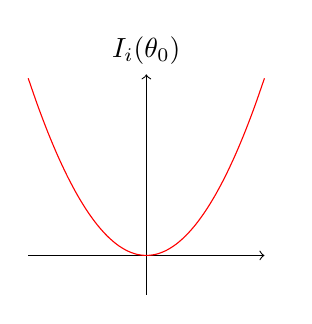
\begin{tikzpicture}
	  \draw[->] (-1.5,0) -- (1.5,0) node[right] {$\mupp$};
      \draw[->] (0,-.5) -- (0, 2.3) node[above] {$I_i(\pars_0)$};
      \draw[scale=1,domain=-1.5:1.5,smooth,variable=\x,red] plot ({\x},{\x*\x});
\end{tikzpicture}
\caption{Fisher information of a point is a parabola of the signal derivative.}
\end{figure}
\begin{figure}[h]\centering
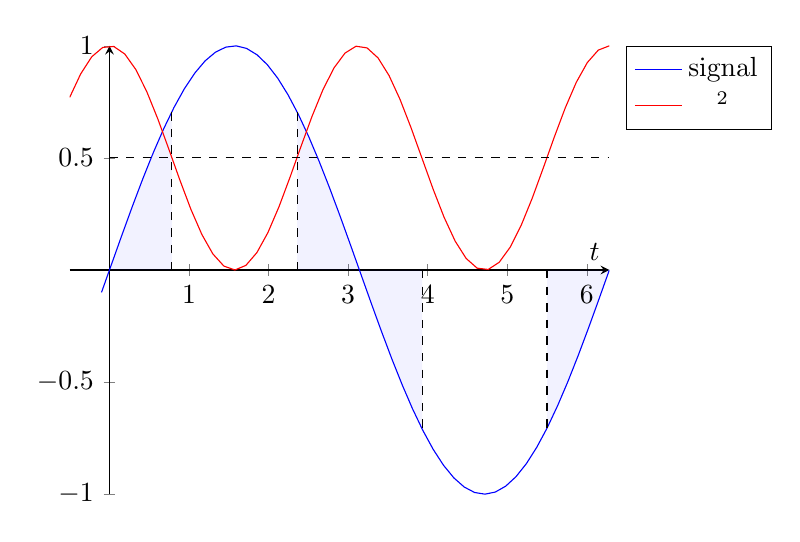
\begin{tikzpicture}
\begin{axis}[axis lines=center, xlabel=$t$, domain=-.5:2*pi, legend pos=outer north east]
	\addplot[color=blue, name path=signal, domain=-.1:2*pi,samples=50] {sin(deg(x))}; \addlegendentry{signal}
	\addplot[color=red, samples=50] {cos(deg(x))^2}; \addlegendentry{$\bkt{\mupp}^2$}
	\addplot[mark=none,dashed, domain=0:2*pi]{.5};
	\draw[dashed] (axis cs:.785,0) -- (axis cs:.785,{sin(deg(.785))});
	\draw[dashed] (axis cs:2.36,0) -- (axis cs:2.36,{sin(deg(2.36))});
	\draw[dashed] (axis cs:3.93,0) -- (axis cs:3.93,{sin(deg(3.93))});
	\draw[dashed] (axis cs:5.5,0) -- (axis cs:5.5,{sin(deg(5.5))});
	\path[name path=axis] (axis cs:0,0) -- (axis cs:2*pi,0);
	\addplot[fill=blue, opacity=.05] fill between [of=signal and axis, soft clip={domain=0:.785}];
	\addplot[fill=blue, opacity=.05] fill between [of=signal and axis, soft clip={domain=2.36:3.93}];
	\addplot[fill=blue, opacity=.05] fill between [of=signal and axis, soft clip={domain=5.5:2*pi}];
\end{axis}     
\end{tikzpicture}
\caption{Filled areas are where the points are more informative.}
\end{figure}

If we attribute each point a weight proportional to its Fisher information, i.e. $w_i = \cos^2(\omega t_i + \phi)$,~\footnote{The variance of $\omega$ is proportional to the (2,2)-minor, in which time doesn't figure, only the squared cosine.} the weight of a region where $\bkt{\mupp}^2 \geq\sfrac12$ is greater than that of an equivalent region with $\bkt{\mupp}^2 < \sfrac12$  by the factor:
\begin{align*}
	\int_{t_0}^{t_1}\cos^2(\omega t + \phi)\rd t = \frac1\omega\int_{\omega t_0}^{\omega t_1} \cos^2\theta\rd\theta = \frac{\Delta t}{2} + \frac{1}{2\omega}\sin\omega\Delta t\cos\omega\Sigma t \approx 1.9.
\end{align*}

The implication is that increasing the number of points measured during the signal's rise and fall is roughly twice as beneficial as doing so during the peaks and troughs.~\footnote{This is not accounting for the fact that
  the certainty of a polarimetry measurement is inversely proportional to its informativity, as was discussed
  in the introduction to this appendix.}

\section{Detector counting rate model}\label{Apx:Stats:Detector_counting_rate}
We assume the following model for the detector counting rate:
\begin{equation}\label{eq:DetCntRt}
	N(t) = N_0(t)\cdot\bkt{1 + P\cdot e^{-\sfrac{t}{\LTd}}\cdot\sin(\omega\cdot t + \phi)},
\end{equation}
where $\LTd$ is the decoherence lifetime, and $N_0(t)$ is the counting rate from the unpolarized cross-section.

Since the beam current can be expressed as a function of time as 
\[
	I(t) \equiv N^b(t)\nu = I_0\cdot e^{\lamb t},
\]
$\lamb$ the beam lifetime, the expected number of particles scattered in the direction of the detector during measurement time $\dtc$ is
\begin{align}
N_0(t) & = p\cdot\int_{-\dtc/2}^{+\dtc/2} I(t+\tau)\rd\tau \notag                    \\
& = p\cdot\frac{\nu N_0^b}{\lamb} e^{\lamb t}\cdot \bkt{e^{\lamb\sfrac{\dtc}{2}} - e^{-\lamb\sfrac{\dtc}{2}}} \notag \\
& \approx \underbrace{p\cdot\nu N_0^b e^{\lamb t}}_{\text{rate}~r(t)} \cdot\dtc,
\end{align}
where $p$ is the probability of ``useful'' scattering (approximately 1\%).

The actual number of detected particles will be distributed as a Poisson distribution
\[
	P_{N_0(t)}(\tilde{N}_0) = \frac{\bkt{r(t)\dtc}^{\tilde{N}_0}}{\tilde{N}_0!}\cdot e^{-r(t)\dtc},
\]
hence $\SD{\tilde{N}_0}^2(t) = N_0(t)$. %In the limit of large $N_0(t)$, one can use the Gaussian approximation.

We are interested in the expectation value $N_0(t) = \Xpct{\tilde{N}_0(t)}$, and its variance $\SD{N_0}(t)$. Those are estimated in the usual way,~\cite{CountRateStat} as 
\begin{align*}
	\avg{\tilde{N}_0(t)}[\dtm] &= \frac{1}{\Ncm}\sum_{i=1}^\Ncm \tilde{N}_0(t_i), ~ \Ncm = \dtm/\dtc,
\shortintertext{and} 
	\SD{\tilde{N}_0(t)}[\dtm] &= \frac{1}{\Ncm}\sum_{i=1}^\Ncm \bkt{\tilde{N}_0(t_i) - \avg{\tilde{N}_0(t_i)}[\dtm]}^2.
\end{align*}
($\dtm$ is the event measurement time, $\dtc$ is the polarimetry measurement time.) A sum of random variables, $N_0(t)$ is normally distributed.

The standard error of the mean then is % abuse of notation here (SD in place of SE) for aesthetic reasons
\begin{align*}
\SD{N_0}(t) & = \SD{\tilde{N}_0}(t)/\sqrt{\Ncm} = \sqrt{N_0(t)\frac{\dtc}{\dtm}}            \\
& \approx \sqrt{\frac{p\cdot\nu N_0^b}{\dtm}}\cdot\dtc \cdot\exp\bkt{\frac{\lamb}{2}\cdot t}.
\end{align*}
\newcommand{\Aa}{\frac{1}{\sqrt{p\cdot\nu N_0^b}}}

Relative error grows:
\begin{equation}\label{eq:MeasRelErr}
	\frac{\SD{N_0}(t)}{N_0(t)} \approx \frac{A}{\sqrt{\dtm}}\cdot\exp\bkt{-\frac{\lamb}{2}t} = \frac{A}{\sqrt{\dtm}}\cdot\exp\bkt{\frac{t}{2\LTb}},~ A=\Aa.
\end{equation}

\section{Cross section asymmetry}
\newcommand{\Asym}{\mathcal{A}}
A measure of the beam's polarization is the relative asymmetry of detector counting rates:~\cite[p.~17]{Eversmann:Thesis}
\begin{equation}\label{eq:AsymDef}
	\Asym = \frac{N(\frac\pi2) - N(-\frac\pi2)}{N(\frac\pi2)+N(-\frac\pi2)}.
\end{equation}

In the simulation to follow, the function fitted to the asymmetry data is:
\begin{equation}\label{eq:xFOM}
	\Asym(t) = \Asym(0)\cdot e^{\lamd\cdot t}\cdot\sin\bkt{\omega\cdot t + \phi},
\end{equation}
with three nuisance parameters $\Asym(0)$, $\lamd$, and $\phi$. 

Due to the decreasing beam size, the measurement of the figure of merit is heteroscedastic. From~\cite[p.~18]{Eversmann:Thesis}, the heteroscedasticity model assumed is
\begin{equation}\label{eq:AsymHtsk}
	\SD{\Asym}^2(t) \approx \frac{1}{2N_0(t)}.
\end{equation}

\section{Measurement time frame}
\DeclareDocumentCommand{\stat}{s}{\IfBooleanTF{#1}{X_{tot}}{\frac{\SD{\meas}^2}{\SE{\hat\omega}^2\cdot \var[w]{t}}}}
\newcommand{\dtnd}{\dt_{zc}}
\newcommand{\SNR}{\text{SNR}}
\newcommand{\deq}{\overset{\triangle}{=}}

Assuming a Gaussian error distribution with mean zero and variance $\SD{\meas}^2$, the maximum likelihood estimator for the variance of the frequency estimate of the cross-section asymmetry $\Asym$ can be expressed as
\begin{align}
\var{\hat\omega} &= \frac{\SD{\meas}^2}{X_{tot}\cdot \var[w]{t}}, \label{eq:VarW}
\shortintertext{with}
X_{tot} &= \sum_{j=1}^{\Nm} x_j = \sum_{s=1}^{\Nnd}\sum_{j=1}^{\Nmnd} x_{js}, \notag\\
\var[w]{t} &= \sum_i w_i \bkt{t_i - \avg{t}[w]}^2,~ \avg{t}[w] = \sum_i w_i t_i, \notag\\
w_i &= \frac{x_i}{\sum_j x_j},~ x_i = (\Asym(0)\exp(\lamd t_i))^2\cos^2(\omega t_i + \phi) = \bkt{\mupp}^2. \notag
\end{align}

In the expression above, $X_{tot}$ is the total Fisher information of the sample, and $\var[w]{t}$ is a measure of its time-spread. It can be observed that by picking appropriate sampling times, one can raise the $X_{tot}$ term, since it is proportional to a sum of the signal's time derivatives. If the oscillation frequency and phase are already known to a reasonable precision, further improvement can be achieved by the application of a sampling scheme in which measurements are taken only during rapid change in the signal (sampling modulation). Improvement here is limited by the polarimetry sampling rate.

Both the $\var[w]{t}$ and $X_{tot}$ terms are bounded as a result of spin tune decoherence. We can express $\sum_{j=1}^{\Nmnd} x_{js} = \Nmnd \cdot x_{0s}$, for some mean value $x_{0s}$ at a given node $s$. $\Nmnd$ is the number of asymmetry measurements per node. The period of time during which measuring takes place, $\dtnd$, is termed \emph{compaction time}. The value of the sum $\sum_{j=1}^{\Nmnd} x_{js}$ falls exponentially due to decoherence, hence $x_{0s} = x_{01}\exp{(\lamd\cdot \frac{(s-1)\cdot\pi}{\omega})}$. Therefore,
\begin{align}
	X_{tot} & = \Nmnd\cdot x_{01} \cdot \frac{\exp{\bkt{\frac{\lamd\pi}{\omega}\Nnd}}-1}{\exp{\bkt{\frac{\lamd\pi}{\omega}}}-1} 
	\equiv \Nmnd \cdot x_{01}\cdot g(\Nnd); \label{eq:FItot}\\
	x_{01}  & = \frac{1}{\dtnd}\int_{-\dtnd/2}^{+\dtnd/2}\cos^2(\omega\cdot t)\rd t = \frac12\cdot \bkt{1 + \frac{\sin\omega\dtnd}{\omega\dtnd}},                                    \label{eq:MeanFIZC}   \\
	\Nmnd   & = \frac{\dtnd}{\dtm}. \label{eq:NumMeasNode}
\end{align}

Eq.~\eqref{eq:FItot} provides us with a means to estimating the limits on the duration of the experiment. In Table~\ref{tbl:FItot}, the percentage of the total Fisher information limit, the time in decoherence lifetimes by which it is reached, and the signal-to-noise ratio by that time, are summarized. The signal-to-noise ratios are computed according to:
\begin{equation}\label{eq:TauRatioSNR}
  \SNR \deq \frac{\Asym(0)\cdot e^{-\sfrac{t}{\LTd}}}{\SD{\Asym}(t)} 
  \approx \sqrt{2\cdot p\cdot\nu N_0^b\cdot \dtc}\cdot \Asym(0)\cdot \exp\bkt*{-\frac{t}{\LTd}\cdot\bkt{1+\frac12\frac{\LTd}{\LTb}}},
  %	 \notag \\
  %	&\approx \Asym(0) \exp\bkt*{-\frac{t}{\LTd}\cdot\bkt{1+\frac12\frac{\LTd}{\LTb}}},
\end{equation}
%in which the factor before $\Asym(0)$ is approximately equal to 1 as a result of: $\SD{N_0}(0)/N_0(0)\approx 3\%$ with 2000 polarimetry measurements per asymmetry measurement ($\dtm = 2000\cdot\dtc$).
in which, from $\SD{\Asym(0)}/\Asym(0) \approx 3\%$, the factor before the exponent is 33.
\begin{table}[h]
  \centering
  \caption{Total Fisher information, by what time it is reached, and the corresponding signal-to-noise ratio.\label{tbl:FItot}}
  \begin{tabular}{rrr}
    \hline
    FI limit (\%) & Reached ($\times\LTd$) &  SNR \\ \hline
    95 &                    3.0 &  0.4 \\
    90 &                    2.3 &  1.1 \\
    70 &                    1.2 &  5.5 \\
    50 &                    0.7 & 11.7 \\ \hline
  \end{tabular}
\end{table}


Eq.~\eqref{eq:VarW} can be rewritten in physical terms assuming zero-decoherence ($\lamd=0$) and uniform sampling with sampling period $\dt$:
\begin{align*}
  \stat* &= \sum_{k=1}^K \Asym^2(0)\cos^2(\omega t_k + \phi) = \frac12 \Asym^2(0)\cdot K, \\
  \var[w]{t} &= \sum_{k=1}^K(k\dt - \avg{t}[w])^2\underbrace{w_k}_{1/K} \\
  &\approx \frac{\dt^2}{12}K^2 = \frac{T^2}{12},
  \intertext{and so}					
  \var{\hat{\omega}} &= \frac{24}{KT^2}\cdot\bkt{\frac{\SD{\meas}}{\Asym(0)}}^2.
\end{align*}

\section{Simulation}
\newcommand{\vp}[2]{{#1}\cdot 10^{#2}}
We simulated data from two detectors with parameters gathered in Table~\ref{tbl:DetCntRtParam} for $T_{tot}=1000$ seconds, sampled uniformly at the rate $f_s = 375$ Hz. These figures are chosen for the following reason: the beam size in a fill is on the order of $10^{11}$ particles; if we want to keep the beam lifetime equal to the decoherence lifetime, we cannot exhaust more than 75\% of it; only 1\% of all scatterings are of the sort we need for polarimetry, so we're left with $\vp{7.5}{8}$ useful scatterings. A measurement of the counting rate $N_0(t)$ with a precision of approximately 3\% requires somewhere in the neighborhood of 2,000 detector counts, which further reduces the number of events to $\vp{3.75}{5}= f_s\cdot T_{tot}$. One thousand seconds is the expected duration of a fill, hence $f_s = 375$ Hz. 

Relative measurement error for the detector counting rates is depicted in Figure~\ref{fig:LRDetErr}; the cross-section asymmetry, computed according to Eq.~\eqref{eq:AsymDef}, is shown in Figure~\ref{fig:Asym}.
To these data we fit via Maximum Likelihood a non-linear heteroscedastic model\footnote{R package nlreg.~\cite{NLREG}} given by Eq.~\eqref{eq:xFOM}, with the variance function for the weights given by Eq.~\eqref{eq:AsymHtsk}. The fit results are summarized in Table~\ref{tbl:FitRes}.
\begin{table}[h]
  \centering
  \caption{Detector counting rates' model parameters\label{tbl:DetCntRtParam}}
  \begin{tabular}{cccc}
    \hline
    &   Left   &     Right     &  \\ \hline
    $\phi$  & $-\pi/2$ &   $+\pi/2$    &   rad   \\
    $\omega$ &  \multicolumn{2}{c}{3}   & rad/sec \\
    $P$    & \multicolumn{2}{c}{0.4}  &  \\
    $\LTd$  & \multicolumn{2}{c}{721}  &   sec   \\
    $\LTb$  & \multicolumn{2}{c}{721}  &   sec   \\
    $N_0(0)$ & \multicolumn{2}{c}{6730} &  \\ \hline
  \end{tabular}
\end{table}

\begin{figure}[h]
  \centering
  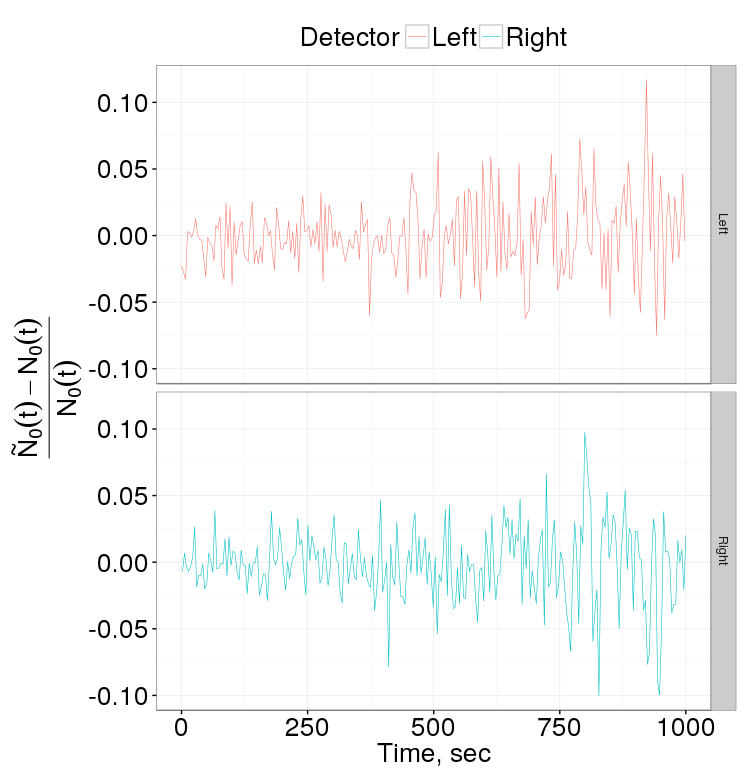
\includegraphics[scale=.85]{images/App_Stats/LR_detector_relErr}
  \caption{Relative counting rate measurement error for the left and right detectors as a function of time.\label{fig:LRDetErr}}
\end{figure}

\begin{figure}[h]
  \centering
  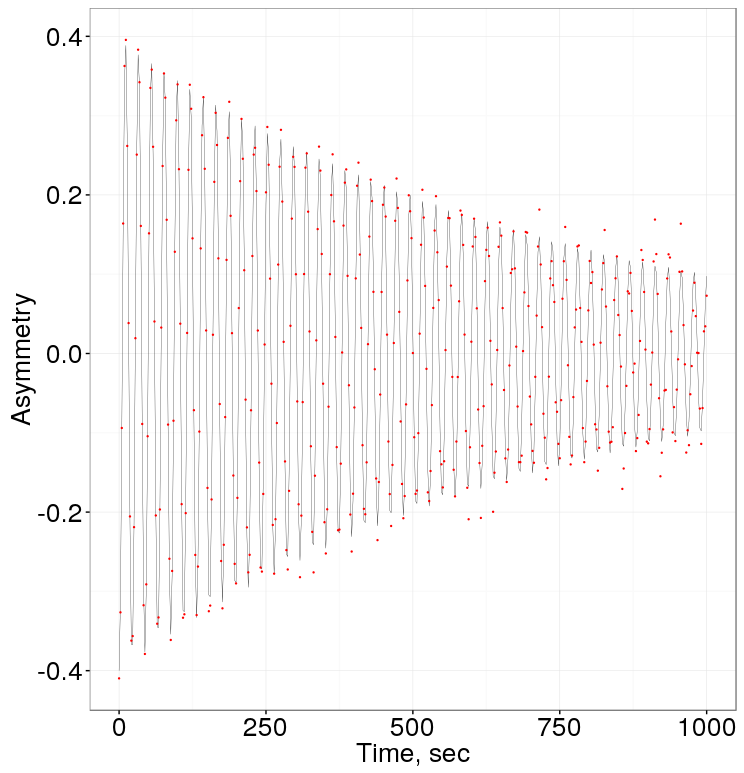
\includegraphics[scale=.85]{images/App_Stats/Asymmetry}
  \caption{Expectation value (red line) and sample measurements (black dots) of the cross-section asymmetry.\label{fig:Asym}}
\end{figure}

\begin{table}[h]
  \centering
  \caption{Fit results\label{tbl:FitRes}}
  \begin{tabular}{crrc}
    \hline
    & Estimate &             SE &  Unit   \\ \hline
    $\Asym(0)$ &   0.400 & $\vp{9.03}{-5}$ &         \\
    $\lamd$   &  -0.001 & $\vp{7.86}{-7}$ &  1/sec  \\
    $\omega$  &   3.000 & $\vp{7.55}{-7}$ & rad/sec \\
    $\phi$   &  -1.571 & $\vp{2.25}{-2}$ &   rad   \\ \hline
  \end{tabular}
\end{table}

If our initial frequency estimate obtained from a time-uniform sample has a standard error on the order of $\vp{1}{-6}$ rad/sec, simulation shows the standard error of the estimate can be improved to $\approx \vp{5.8}{-7}$ rad/sec.
